

\subsection{クライアントサイドの実装}\label{4.1.2}
クライアントサイドでは,WebAPIを利用して,Webアプリケーションを実装した.
Webアプリケーションのフレームワークとして,Next.jsを採用した.
Next.jsはReact.jsをベースにしており,React.jsの開発を効率化に加え,サーバーサイドによるレンダリングをサポートによるSEO対策やパフォーマンスの向上を実現できる.
React.jsはJavaScriptのライブラリであり,コンポーネントベースのアーキテクチャを採用している.
コンポーネントを独立した単位として開発すると,開発者はそれぞれのコンポーネントに集中できるため開発効率が向上する.
コンポーネントは再利用可能な単位であり複数のページで同じコンポーネントを利用することができ,これにより開発コストを削減し保守性を向上させる.
またReactは仮想DOMを採用しており実際のDOM(Document Object Model)を操作する代わりに、JavaScriptのオブジェクトとして扱う仕組みである.
仮想DOMは実際のDOMと比較して,更新が必要な部分だけを計算を行うためパフォーマンスの向上が図れる.



基本的に既存の滞在ウォッチで同じように滞在者,滞在画面,利用者情報のページが存在する.
変更点として滞在時間をガントチャートで可視化している画面が挙げられる.
\ref{fig:gantt}にその画面を示す.
この画面の緑の部分にカーソルを合わせると,入室時間と退室時間を確認できる.
日付と部屋を指定するタブがあり,そのタブに応じたそれぞれのデータを表示される.

\begin{figure}[tbh]
  \centering
  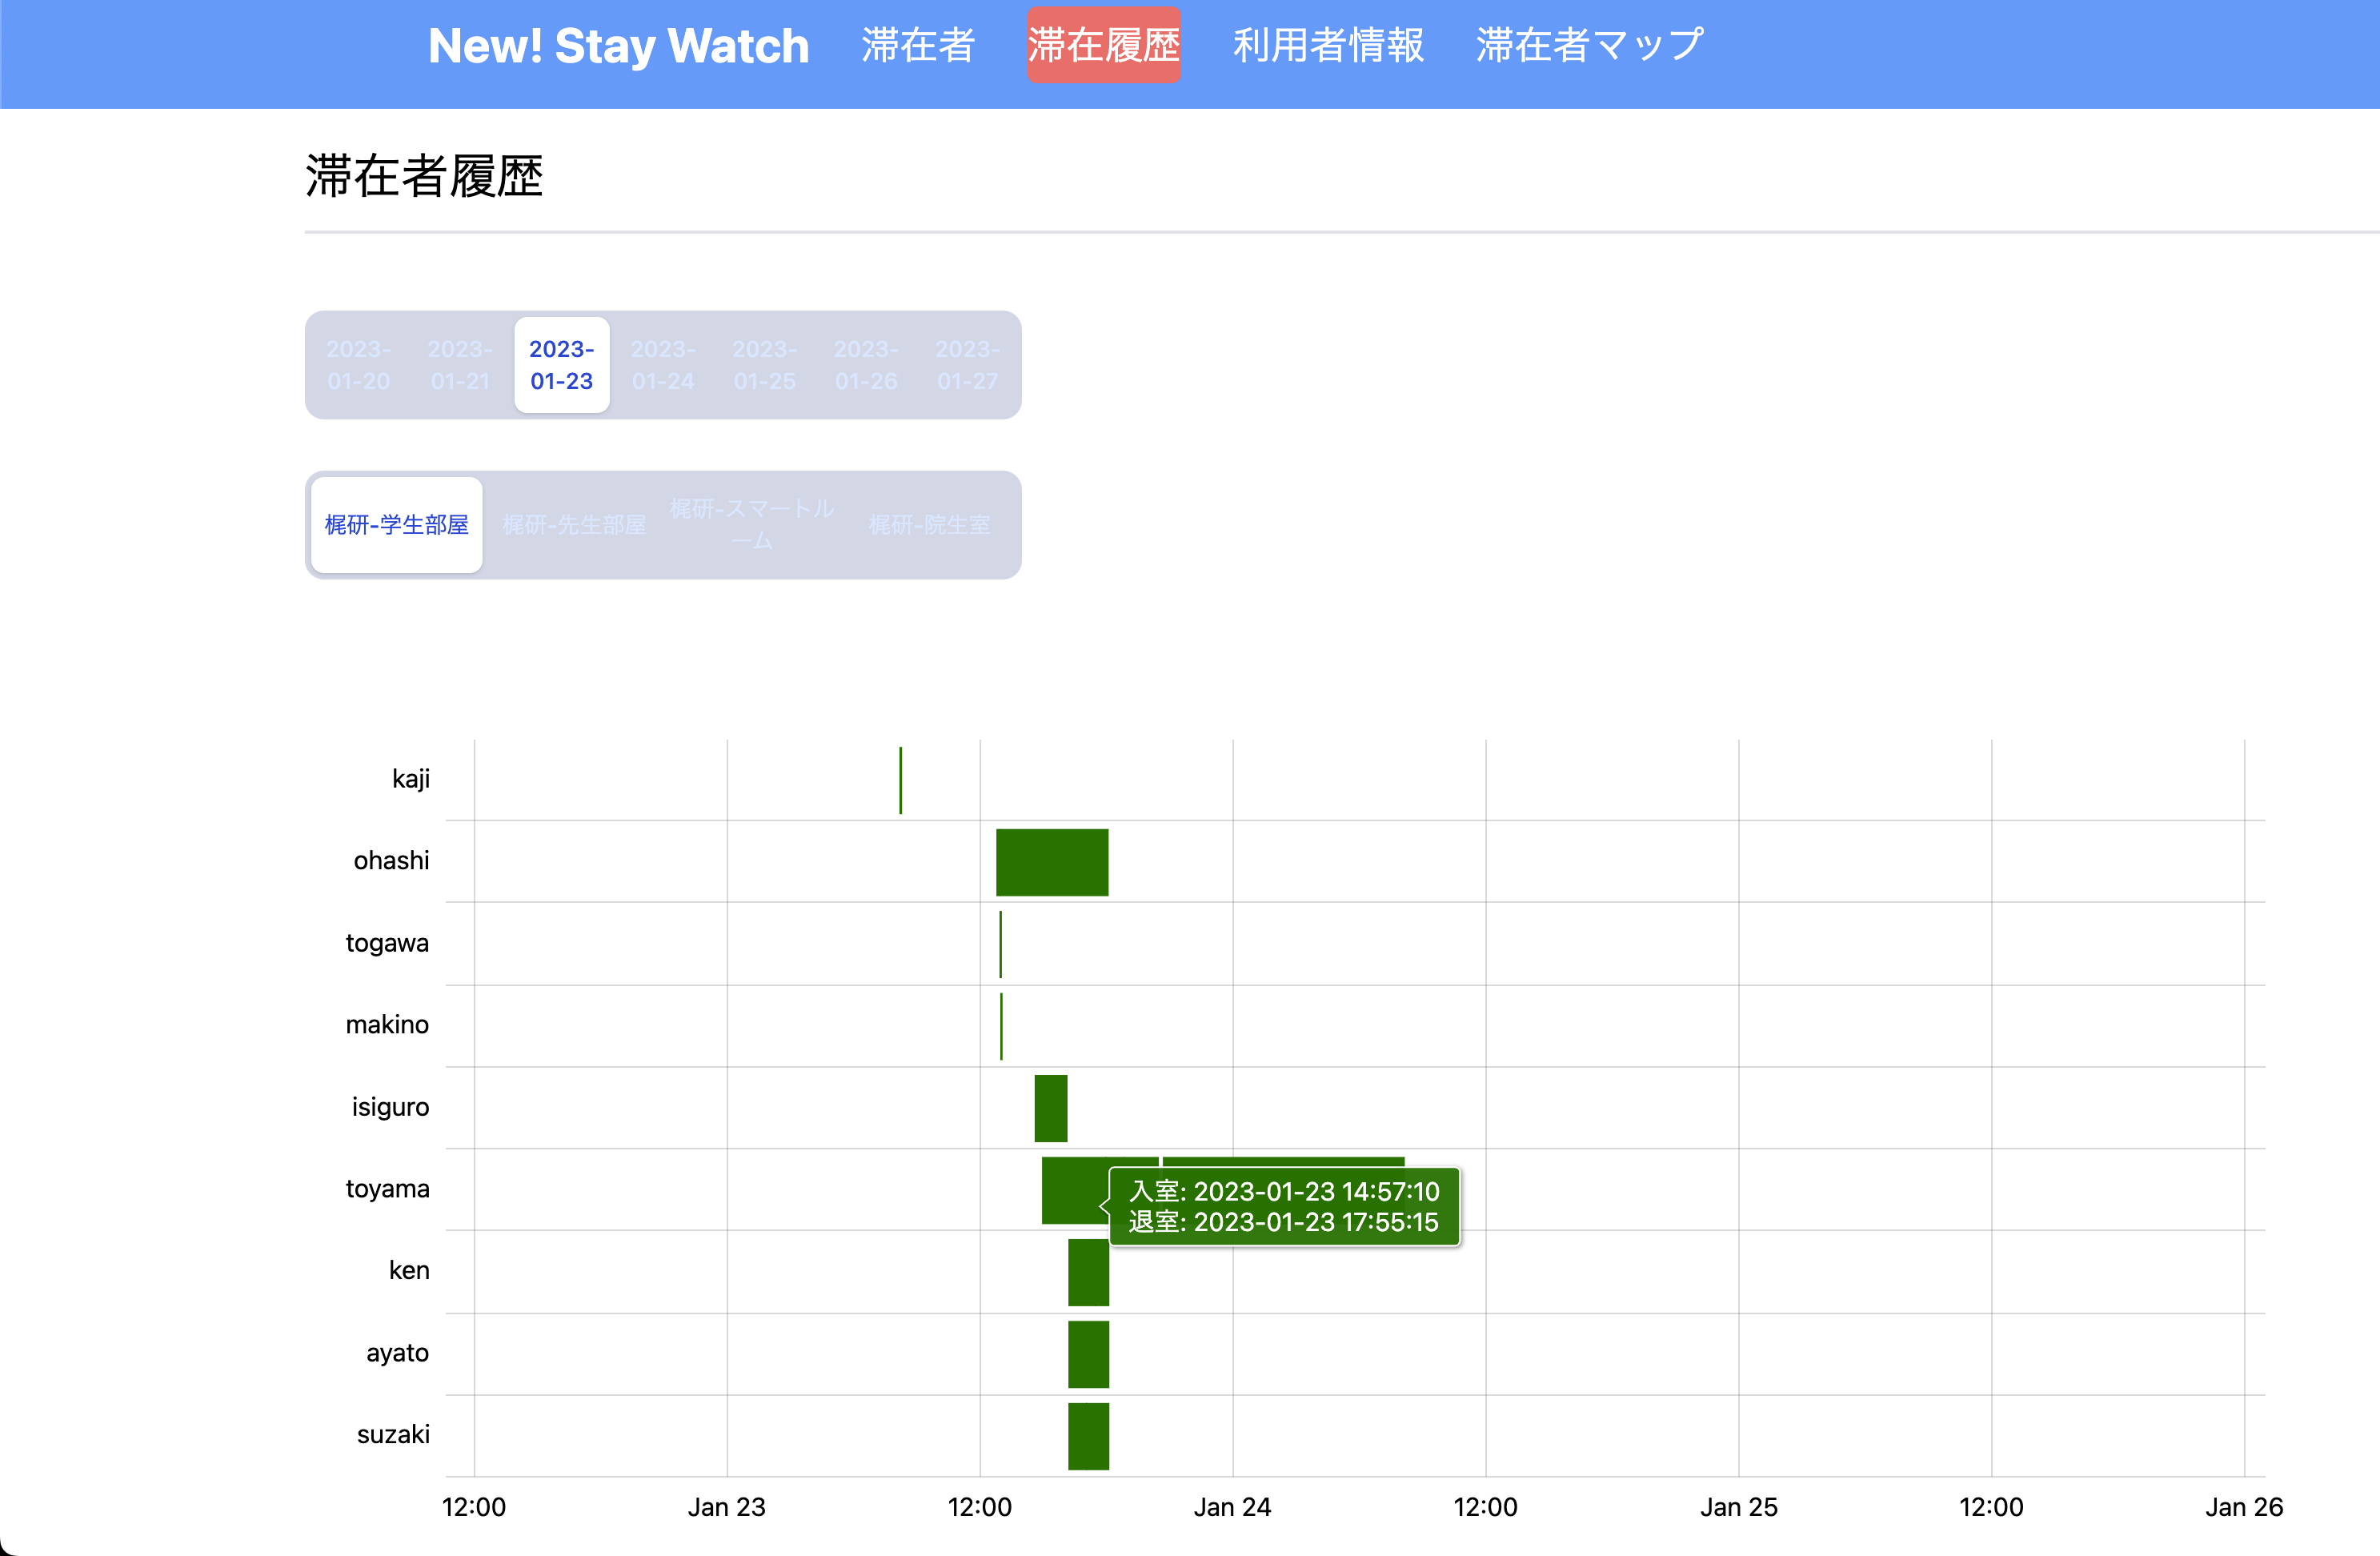
\includegraphics[width=16cm]{image/gantt.jpg}
  \caption{ガントチャートを用いた滞在時間の可視化} \label{fig:gantt}
\end{figure}













